\chapter{Il modello lineare}
\label{chapter:stat_models} 


%--------------------------------------------------------------------
 
Prima di descrivere come il modello di regressione lineare possa essere applicato ai dati, esamineremo i modelli statistici Bayesiani che vengono utilizzati in alcuni casi più semplici, ovvero (1) il modello statistico per una proporzione e (2) il modello statistico utilizzato per il confronto tra due proporzioni.
Estenderemo poi la discussione al caso in cui viene considerato (3) un campione di osservazioni misurate su scala continua, assumendo che ciascuna osservazione provenga da una distribuzione Normale.
In tali circostanze, l'oggetto dell'inferenza sarà il parametro $\mu$ che rappresenta la media della popolazione da cui le osservazioni sono state tratte.
A questo punto saremo nelle condizioni di discutere (4) l'inferenza Bayesiana sulla differenza tra le medie di due popolazioni.
Tale problema verrà affrontato specificando un modello di regressione lineare che include una variabile dipendente continua e una variabile indipendente dicotomica.
Una volta chiarite le proprietà del modello di regressione in questo caso semplice, sarà immediato estendere la discussione (5) al caso di una variabile indipendente continua.


\section{Modello Binomiale}

Se facciamo nuovamente riferimento all'esempio del capitolo~\ref{chapter:likelihood}, nel quale abbiamo osservato $A = 6$ volte \enquote{acqua} in $N = 9$ prove Bernoulliane indipendenti, allora il modello statistico che descrive l'esperimento casuale può essere formulato nei termini seguenti:
\begin{align}
A &\sim \text{Binomiale}(N, p) \tag*{[verosimiglianza]}\\
p &\sim \text{Uniforme}(0, 1) \tag*{[distr. a priori per $p$]}
\end{align}
dove la prima riga definisce la funzione di verosimiglianza e la seconda riga definisce la distribuzione a priori.
Il segno $\sim$ (tilde) si può leggere \enquote{si distribuisce come}.
La prima riga, dunque, ci dice che la variabile aleatoria $Y$ segue la distribuzione Binomiale di parametri $N$ e $p$.
La seconda riga specifica che, quale distribuzione a priori, assumiamo una distribuzione uniforme in (0 e 1) per il parametro $p$.


\section{Il presidente Trump e l'idrossiclorochina}
\label{sec:idrossi}

Cito dal \emph{Washington Post} del 7 aprile 2020:
\begin{quote}
\enquote{One of the most bizarre and disturbing aspects of President Trump's nightly press briefings on the coronavirus pandemic is when he turns into a drug salesman. 
Like a cable TV pitchman hawking \enquote{male enhancement} pills, Trump regularly extols the virtues of taking hydroxychloroquine, a drug used to treat malaria and lupus, as a potential \enquote{game changer} that just might cure covid-19.}
\end{quote} 
Tralasciamo qui il fatto che il presidente Trump non è un esperto in questo campo. 
Esaminiamo invece le evidenze iniziali a supporto dell'ipotesi che l'idrossiclorochina possa essere utile per la cura del Covid-19, evidenze disponibili nel momento in cui il presidente Trump ha fatto le affermazioni riportate sopra.\footnote{In seguito, quest'idea è stata completamente screditata.}
Tali evidenze sono state fornite 
%in un articolo dal titolo \enquote{Hydroxychloroquine and azithromycin as a treatment of COVID-19: results of an open-label non-randomized clinical trial} pubblicato su 
%\emph{International Journal of Antimicrobial Agents} 
da \citet{Gautret_2020}. 

Il disegno sperimentale di \citet{Gautret_2020} comprende, tra le altre cose, il confronto tra una condizione sperimentale e una condizione di controllo.
Un articolo pubblicato da \citet{Hulme_2020} si è posto il problema di rianalizzare i dati di \citet{Gautret_2020} -- si veda \url{https://osf.io/5dgmx/}.
Tra gli autori di questo secondo articolo figura anche Eric-Jan Wagenmakers, uno psicologo molto conosciuto per i suoi contributi metodologici.
%L'analisi proposta da \citet{Hulme_2020} è di tipo Bayesiano, per questa ragione la cito qui.
%Nell'Abstract, \citet{Hulme_2020} riportano quanto segue:
%\begin{quote}
%\enquote{Our analyses only explore the effects of different assumptions about excluded and untested patients. These assumptions are not adequately reported, nor are they justified in the original paper, and we find that varying them causes substantive changes to the evidential support for the main claims of the original paper.}
%\end{quote} 
\citet{Hulme_2020} sottolineano il fatto che \citet{Gautret_2020} si sono concentrati, nella loro analisi dei dati, soltanto su una parte del loro campione. 
Se però vengono considerati anche i pazienti che sono stati esclusi dall'analisi dei dati, le conclusioni a cui sono giunti \citet{Gautret_2020} risultano fortemente indebolite.

L'analisi dei dati proposta da \citet{Hulme_2020} richiede l'uso di alcuni strumenti statistici che, in queste dispense, non verranno discussi.  
Ma possiamo giungere alle stesse conclusioni di \citet{Hulme_2020} anche usando le procedure statistiche che abbiamo descritto finora.
%Utilizziamo qui i dati riportati da \citet{Gautret_2020} per fare un esercizio didattico nel quale esamineremo le funzionalità del pacchetto \verb+rethinking+, senza avere l'ambizione di entrare nel merito di questa discussione. 
%Ciò non toglie il fatto che, anche usando la procedura descritta di seguito, saremo in grado di arrivare alle stesse conclusioni proposte da \citet{Hulme_2020}.
%Iniziamo con il caricare il pacchetto \verb+rethinking+:
%\begin{lstlisting}
%library("rethinking")
%\end{lstlisting}
Nella ricerca di \citet{Gautret_2020} il confronto importante è tra la proporzione di paziente positivi al virus SARS-CoV-2 nel gruppo a cui è stata somministrata l'idrossiclorochina (6 su 14) e nel gruppo di controllo (a cui non è stata somministrata l'idrossiclorochina: 14 positivi su 16). 
Ciò che faremo sarà di calcolare la distribuzione a posteriori per queste due proporzioni.
Rappresenteremo graficamente le due distribuzioni a posteriori per il parametro $p$ che rappresenta la probabilità di risultare positivo al SARS-CoV-2.
Calcoleremo anche, separatamente per i due gruppi, l'intervallo di credibilità al 95\%.
Quindi concluderemo facendo il confronto tra gli intervalli di credibilità dei due gruppi.

Leggiamo i dati in R\, creando i due vettori seguenti.
Il vettore \verb+ym+ contiene i dati del gruppo a cui è stata somministrata l'idrossiclorochina e il vettore \verb+yc+ i dati del gruppo di controllo.
Il valore $y = 1$ indica che il paziente è positivo al virus SARS-CoV-2 (l'ordine di 0 e 1 è irrilevante).
\begin{lstlisting}
ym <- c(rep(1, 6), rep(0, 8))
ym
#> [1] 1 1 1 1 1 1 0 0 0 0 0 0 0 0
yc <- c(rep(1, 14), rep(0, 2))
yc
#> [1] 1 1 1 1 1 1 1 1 1 1 1 1 1 1 0 0
\end{lstlisting}
\noindent
Utilizzando la sintassi di \verb+rethinking+, definiamo ora il modello statistico per una proporzione specificando una distribuzione a priori non informativa:
\begin{lstlisting}
flist <- alist(
  y ~ dbinom(1, p),
  p ~ dbeta(1, 1) 
)
\end{lstlisting}
\noindent
Calcoliamo la distribuzione a posteriori per il parametro $p$ nel caso del gruppo sperimentale
\begin{lstlisting}
m <- quap( 
  flist, 
  data = list(y = ym)
)
\end{lstlisting}
\noindent
e troviamo l'intervallo di credibilità al 95\%:
\begin{lstlisting}
precis(m, prob = 0.95)
#>   mean   sd 2.5% 97.5%
#> p 0.43 0.13 0.17  0.69
\end{lstlisting}
\noindent
Creiamo poi un grafico della distribuzione a posteriori per $p$:
\begin{lstlisting}
post <- extract.samples(m)
plot(
  density(post$p), 
  xlim = c(0, 1),
  ylim = c(0, 5),
  main = "",
  xlab = "Parametro p",
  ylab = "Densita'"
)
\end{lstlisting}
\noindent
Ripetiamo ora la stessa procedura usando però i dati del gruppo di controllo.
Disegniamo quindi la nuova distribuzione a posteriori per $p$ nello stesso grafico creato in precedenza:
\begin{lstlisting}
m <- quap( 
  flist, 
  data = list(y = yc)
)
precis(m, prob = 0.95)
#>   mean   sd 2.5% 97.5%
#> p 0.87 0.08 0.71  1.04
post <- extract.samples(m)
lines(density(post$p), xlim = c(0, 1))
\end{lstlisting}

\begin{figure} %[h!]
 \centering
 \includegraphics[width=0.8\textwidth]{trump_covid19}
 \caption{Distribuzioni a posteriori del parametro $p$ che rappresenta la probabilità di risultare positivo al virus SARS-CoV-2 per i due gruppi di pazienti considerati nella ricerca di \citet{Gautret_2020}.
}
\label{fig:trump_covid19}
\end{figure}

Come evidenziato dalla figura~\ref{fig:trump_covid19}, le distribuzioni a posteriori per il parametro $p$  sono abbastanza separate, il che suggerisce che il parametro $p$ assume valori diversi nel caso dei due gruppi.
Coerentemente con la conclusioni di \citet{Gautret_2020}, le nostre stime a posteriori per il parametro $p$ suggeriscono dunque che i pazienti del gruppo sperimentale (a cui è stata somministrata l'idrossiclorochina) hanno una minore probabilità di risultare positivi al SARS-CoV-2 che i pazienti del gruppo di controllo (a cui non è stata somministrata l'idrossiclorochina). 

A questa conclusione possiamo anche giungere confrontando gli intervalli di credibilità al 95\% dei due gruppi.
Gli intervalli di credibilità non si sovrappongono, il che suggerisce che il valore del parametro $p$ è diverso nei due gruppi.
Possiamo dunque concludere, con un grado di certezza soggettiva del 95\%, che nel gruppo sperimentale vi è una probabilità più bassa di risultare positivi al SARS-CoV-2 che nel gruppo di controllo.
Fino a qui non abbiamo fatto altro che replicare le conclusioni a cui sono giunti \citet{Gautret_2020}, sia pur utilizzando una procedura statistica diversa.

\citet{Hulme_2020} mettono però in evidenza il fatto che \citet{Gautret_2020}, nella loro analisi statistica, hanno escluso alcuni pazienti che, nel gruppo sperimentale, sono in realtà peggiorati, anziché essere migliorati. 
Se consideriamo i dati di tutti i pazienti del campione (non solo quelli selezionati da \citet{Gautret_2020}, la situazione è la seguente. 
Gruppo sperimentale: 10 positivi su 18; gruppo di controllo: 14 positivi su 16.
Ripetiamo dunque l'analisi descritta sopra utilizzando, per il gruppo sperimentale, i dati appena descritti.
Così facendo otteniamo il seguente intervallo di credibilità al 95\%:


\begin{lstlisting}
ym <- c(rep(1, 10), rep(0, 8))
ym
#> [1] 1 1 1 1 1 1 1 1 1 1 0 0 0 0 0 0 0 0
m <- quap( 
  flist, 
  data = list(y = ym)
)
precis(m, prob = 0.95)
#>   mean   sd 2.5% 97.5%
#> p 0.56 0.12 0.33  0.79
\end{lstlisting}



\noindent
In queste circostanze notiamo che l'intervallo di credibilità al 95\% per il gruppo sperimentale, ovvero [0.33, 0.79], si sovrappone all'intervallo di credibilità al 95\% per il gruppo di controllo, ovvero [0.71  1.04]. 
In base agli standard correnti, un risultato di questo tipo non viene considerato come evidenza sufficiente per potere concludere che il parametro $p$ differisce tra i due gruppi.

Concludiamo dicendo che questo, ovviamente, è solo un esercizio didattico: la ricerca di \citet{Gautret_2020} include tante altre informazioni che qui non sono state considerate.
Tuttavia, notiamo che la semplice analisi statistica che abbiamo descritto è stata in grado di replicare le conclusioni a cui sono giunti (per altra via) \citet{Hulme_2020}.
% Ciò dovrebbe fare riflettere.
% Chissà, forse il presidente Trump potrebbe aggiungere qualche considerazione statistica interessante a questo nostro esercizio didattico.


\section{Modello Normale}

Facciamo ora un altro esempio considerando, in questo caso, la distribuzione Normale descritta nella sezione~\ref{sec:bdi2_30_sogg}:
\begin{align}
Y_i &\sim \mathcal{N}(\mu, \sigma) \tag*{[verosimiglianza]}\\
\mu &\sim \mathcal{N}(\mu = \bar{X}, \sigma = 100) \tag*{[distr. a priori per $\mu$]}\\
\sigma &= s_Y \tag*{[parametro assunto noto]}
\end{align}
Questo secondo modello statistico ci dice che la variabile aleatoria $Y$ segue la distribuzione Normale di parametri $\mu$ e $\sigma$. 
Il parametro $\mu$ è sconosciuto e abbiamo deciso di descrivere la nostra incertezza a priori relativa ad esso mediante una distribuzione a priori che segue la legge Normale con media uguale alla media campionaria e deviazione standard 100.
Il parametro $\sigma$ è fissato ad un valore pari alla deviazione standard del campione, $s_y$.
In generale, però, anche il parametro $\sigma$ viene considerato ignoto e ad esso potrebbe essere assegnata una distribuzione a priori come, ad esempio, $\sigma \sim \text{Unif}(0, 100)$.


%--------------------------------------------------------------------
\subsection{Il modello normale con \texttt{quap()}}

I valori del BDI-II dei 30 soggetti clinici del campione di \citet{zetsche_future_2019} sono:



\begin{lstlisting}
26 35 30 25 44 30 33 43 22 43 24 19 39 31 25 28 35 
30 26 31 41 36 26 35 33 28 27 34 27 22
\end{lstlisting}
 


\noindent
Calcoliamo le statistiche descrittive:



\begin{lstlisting}
true_sd <- sd(df$x)
true_sd
#> 6.606858

sample_mean <- mean(df$x)
sample_mean
#> 30.93333
\end{lstlisting}
 


\noindent
Definiamo il modello statistico mediante \verb+alist()+:




\begin{lstlisting}
flist <- alist(
  x ~ dnorm(mu, sigma), 
  mu ~ a,
  a ~ dnorm(sample_mean, 100),
  sigma ~ true_sd
)
\end{lstlisting}
 


\noindent
Calcoliamo la distribuzione a posteriori:


\begin{lstlisting}
m1 <- quap( 
   flist,
   data = df 
)
\end{lstlisting}
 


\noindent
Esaminando il risultato mediante \verb+precis()+




\begin{lstlisting}
   mean   sd  2.5% 97.5%
a 30.93 1.21 28.57  33.3
\end{lstlisting}
 


\noindent
stabiliamo che l'intervallo di credibilità al 95\% per il valore medio del BDI-II è [28.57, 33.3].
Questo esempio mostra dunque come calcolare l'intervallo di credibilità nel caso della media di un campione.
Nella sezione successiva ci porremo il problema di fare il confronto tra le medie di due campioni indipendenti. 


%--------------------------------------------------------------------
\section{Il modello di regressione lineare}
\label{sec_mod_lin}

I due modelli statistici precedenti descrivono il comportamento di una singola variabile aleatoria: una proporzione di \enquote{successi} o la media del livello BDI-II in un campione clinico.
Tuttavia, i modelli di interesse per la psicologia (e per le altre scienze) descrivono le relazioni tra due o più variabili.
Nel suo studio \emph{Regression towards mediocrity in hereditary stature}  Galton (1886) si chiesto quale relazione intercorre tra l'altezza dei figli e l'altezza dei padri.
Il modo più semplice per rispondere ad una domanda di questo tipo è quello di formulare la risposta nei termini di un \emph{modello di regressione lineare} (appunto, la tecnica statistica che è stata proposta da Galton). 
Il modello di regressione lineare è il più semplice dei modelli statistici che descrivono la relazione tra due (o più) variabili e, probabilmente, anche il più usato.
Tale modello può essere descritto nel modo seguente:
\begin{align}
Y_i &\sim \mathcal{N}(\mu_i, \sigma) \tag*{[verosimiglianza]}\\
\mu_i &= \alpha + \beta(X_i - \bar{X}) \tag*{[modello lineare]}\\
\alpha &\sim \mathcal{N}(0, \sigma_{\alpha}) \tag*{[distr. a priori per $\alpha$]}\\
\beta &\sim \mathcal{N}(0, \sigma_{\beta}) \tag*{[distr. a priori per $\beta$]}\\
\sigma &\sim \text{Uniforme}(0, 50) \tag*{[distr. a priori per $\sigma$]}
\end{align}
La verosimiglianza indica che ciascun valore $Y_i$ (la nostra variabile dipendente) segue una distribuzione Normale.
Tuttavia, ciascuna $Y_i$ segue una distribuzione Normale avente una media diversa (come indicato dal pedice $i$ usato per $\mu_i$).
In questa formulazione del modello, tutte le distribuzioni Normali relative alla $Y$ hanno la stessa deviazione standard.
La cosa importante è che la media $\mu$ non è più il parametro che deve essere stimato -- come avveniva invece nel caso del modello Normale per i valori BDI-II.
Nel modello statistico della regressione lineare, invece, $\mu_i$ è espresso nei termini di due altri parametri, $\alpha$ e $\beta$, e di una quantità osservabile chiamata $X$ (la variabile indipendente).
La seconda riga del modello non esprime una relazione stocastica (non viene usato il segno $\sim$), ma bensì una relazione deterministica (come indicato dal segno di uguale). 
Ciò significa che, una volta fissati i parametri $\alpha$ e $\beta$, il valore $\mu_i$ è determinato in maniera univoca.
Se il modello di regressione lineare è espresso come $\mu_i = \alpha + \beta(X_i - \bar{X})$, allora possiamo assegnare ai parametri $\alpha$ e $\beta$ la seguente interpretazione:
\begin{enumerate}
\item
il parametro $\alpha$ è uguale alla media della $Y$;
\item
il parametro $\beta$ ci dice quanto varia, in media, il valore $Y$ per ogni variazione unitaria della $X$.
Il parametro $\beta$ viene chiamato \enquote{pendenza} perché, in termini geometrici, il modello di regressione lineare assume la forma di una retta che, all'interno di un diagramma a dispersione, approssima quanto meglio è possibile la nube di punti $(X, Y)$.
\end{enumerate}


%--------------------------------------------------------------------
\subsection{Variabile indipendente dicotomica}
\label{sec_var_ind_dico}

Solitamente, in un modello lineare come quello descritto nella \S~\ref{sec_mod_lin}, la variabile $X$ è una variabile continua, ma potrebbe anche essere una variabile discreta.
Nel caso più semplice, $X$ assume solo due valori: 0 e 1.
In tali circostanze, il modello lineare può essere usato per il confronto tra le medie di due gruppi.

Se $X$ è una variabile dicotomica (con valori 0 e 1), per il modello lineare $\mu_i = \alpha + \beta x_i$ abbiamo quanto segue: quando $X=0$, $\mu_i = \alpha$ e, quando $X=1$, $\mu_i = \alpha + \beta$.
Ciò significa che il parametro $\alpha$ è uguale alla media del gruppo codificato con $X=0$ e 
il parametro $\beta$ è uguale alla differenza tra le medie dei due gruppi (essendo la media del secondo gruppo uguale a $\alpha + \beta$).

In tali circostanze, il parametro $\beta$ risulta particolarmente utile in quanto, nel caso di due gruppi, può essere usato per codificare l'effetto di una manipolazione sperimentale o di un trattamento.
Per \enquote{effetto di un trattamento} si intende appunto la differenza tra le medie di due gruppi (talvolta, il gruppo \enquote{sperimentale} e il gruppo \enquote{di controllo}).
L'inferenza su $\beta$ può dunque aiutarci a capire quanto può essere considerato \enquote{robusto} l'effetto di un trattamento o di una manipolazione sperimentale.


%--------------------------------------------------------------------
\subsection{Un esempio pratico}
\label{sec_var_ind_dico}

Esaminiamo un sottoinsieme di dati tratto dal \emph{National Longitudinal Survey of Youth} e discusso da Gelman, Hill e Vehatari (2020).
I soggetti sono bambini di 3 e 4 anni.
La variabile dipendente, \texttt{kid\_score}, è il punteggio totale del \emph{Peabody Individual Achievement Test} (PIAT) costituito dalla somma dei punteggi di tre sottoscale (Mathematics, Reading comprehension, Reading recognition). 
La variabile indipendente, \texttt{mom\_hs}, è il livello di istruzione della  madre, codificato con due livelli: scuola media superiore completata oppure no.
La domanda della ricerca è se il QI del figlio (misurato con la scala PIAT) risulta associato al livello di istruzione della madre.

Codifichiamo il livello di istruzione della madre ($X$) con una \emph{variabile indicatrice} (ovvero, una variabile che assume solo i valori 0 e 1) tale per cui:
\begin{itemize}
\item $X=0$: la madre non ha completato la scuola secondaria di secondo grado (scuola media superiore);
\item $X=1$: la madre ha completato la scuola media superiore.
\end{itemize}
Il punteggio PIAT medio è 77.55 per il gruppo di bambini la cui madre non ha il diploma di scuola media superiore, e pari a 89.32 per il gruppo di bambini la cui madre ha completato la scuola media superiore.
Questa differenza suggerisce un'associazione tra le variabili, ma tale differenza potrebbe essere soltanto la conseguenza della variabilità campionaria, senza riflettere una caratteristica generale della popolazione.
Come possiamo usare il modello statistico lineare per fare inferenza sulla differenza osservata tra i due gruppi?

Supponiamo che i dati siano contenuti nel data.frame \verb+df+.
Calcoliamo le statistiche descrittive per i due gruppi:




\begin{lstlisting}
df %>% 
  group_by(mom_hs) %>% 
  summarise(
    mean_kid_score = mean(kid_score),
    std = sqrt(var(kid_score))
  )

#>   mom_hs mean_kid_score   std
#> 1      0          77.55 22.57
#> 2      1          89.32 19.05
\end{lstlisting}
 


Specifichiamo ora il modello statistico che descrive la differenza tra i punteggi PIAT dei due gruppi in base ad un modello di regressione lineare:




\begin{lstlisting}
flist <- alist(
  kid_score ~ dnorm(mu, sigma),
  mu ~ a + b * mom_hs,
  a ~ dnorm(86.8, 100),
  b ~ dnorm(0, 100),
  sigma ~ dunif(0, 100)
)
\end{lstlisting}
 


Si noti che abbiamo specificato il modello statistico seguendo la stessa procedura descritta all'inizio della \S~\ref{sec_mod_lin}.
Ovvero, abbiamo descritto in maniera esplicita:
\begin{itemize}
\item la verosimiglianza dei dati,
\item il modello statistico della regressione lineare che esprime il valore atteso della variabile dipendente come una funzione lineare della variabile indipendente,
\item la distribuzione a priori di ciascuno dei parametri del modello, ovvero $a$, $b$ e $\sigma$.
\end{itemize}

Abbiamo specificato due distribuzioni a priori \enquote{debolmente informative} per i parametri $a$ e $b$.
La distribuzione a priori del parametro $a$ è una distribuzione Normale centrata sulla media di tutti i dati (calcolata ignorando la suddivisione in gruppi), con una deviazione standard relativamente grande. 
Ciò significa che, per il parametro $a$, a priori noi riteniamo plausibili valori che vanno da circa $86.8 \pm 2 \times 100$ punti PIAT, anche se riteniamo più probabili i valori prossimi alla media generale pari a 86.8.
Così facendo, \emph{prima} di avere osservato i dati campionari, esprimiamo una generale incertezza su quello che potrebbe essere il valore della media del gruppo codificato con $X = 0$.

In maniera simile, caratterizziamo il possibile valore della differenza tra le medie tra i due gruppi (ciò a cui siamo interessati) in maniera molto vaga: affermiamo che potrebbe essere un valore qualsiasi, probabilmente contenuto nell'intervallo $0 \pm 2 \times 100$, assegnando a priori una plausibilità maggiore ai valori prossimi allo zero (positivi e negativi).
Per il parametro $b$, specifichiamo una distribuzione a priori Normale centrata sullo zero.
Così facendo, la distribuzione a priori non favorisce né l'ipotesi secondo cui il parametro $b$ è maggiore di zero (ovvero, la media dei punteggi PIAT è maggiore nel gruppo codificato con $X = 0$ rispetto al gruppo codificato con $X = 1$), né  l'ipotesi opposta.
Specificando per $b$ una distribuzione a priori simmetrica centrata sullo zero non introduciamo dunque alcuna distorsione nella distribuzione a posteriori; non favoriamo dunque né l'ipotesi a cui potremmo essere interessati (ad esempio, $a > 0$) né l'ipotesi opposta.

Infine, specifichiamo distribuzione a priori uniforme nell'intervallo (0, 100) per il  parametro $\sigma$ che descrive la distribuzione dei dati attorno al loro valore atteso.

Adattiamo il modello ai dati utilizzando la funzione \verb+quap()+ del pacchetto \verb+rethinking+: 
\begin{lstlisting}
m1 <- quap(
  flist,
  data = df
)
\end{lstlisting}
 


\noindent
Estraiamo alcuni campioni dalla distribuzione a posteriori:




\begin{lstlisting}
post <- extract.samples(m1)
post[1:5, ]

#>          a         b    sigma
#> 1 80.81017 11.304323 19.91794
#> 2 76.04906 12.298966 19.57723
#> 3 80.53425  8.668147 19.67729
#> 4 76.83047 13.067251 20.18224
#> 5 80.62879  8.110674 19.51875
\end{lstlisting}
 


\noindent
Esaminiamo la distribuzione a posteriori dei parametri mediante le seguenti istruzioni:




\begin{lstlisting}
par(mfrow = c(1, 3))
dens(
  post$a,
  col = rangi2, lwd = 2.5, xlab = "",
  ylab = "Densita'", main = "p(a | x, y)",
  cex.lab = 1.5, cex.axis = 1.35, cex.main = 1.5,
  cex.sub = 1.5
)
dens(
  post$b,
  col = rangi2, lwd = 2.5, xlab = "",
  ylab = "", main = "p(b | x, y)",
  cex.lab = 1.5, cex.axis = 1.35, cex.main = 1.5,
  cex.sub = 1.5
)
dens(
  post$sigma,
  col = rangi2, lwd = 2.5, xlab = "",
  ylab = "", main = "p(sigma | x, y)",
  cex.lab = 1.5, cex.axis = 1.35, cex.main = 1.5,
  cex.sub = 1.5
)
par(mfrow = c(1, 1))
\end{lstlisting}
 


\noindent
Il risultato viene mostrato nella figura~\ref{fig:kid_score_mom_hs_post_distr}.

\begin{figure} %[h!]
 \centering
 \includegraphics[width=\textwidth]{kid_score_mom_hs_post_distr}
 \caption{Distribuzione a posteriori dei parametri $a$, $b$ e $\sigma$ del modello statistico lineare che descrive i punteggi del \emph{Peabody Individual Achievement Test} come funzione del gruppo di appartenenza: i bambini la cui madre non ha completato la scuola media superiore e i bambini la cui madre ha completato la scuola media superiore.
I dati sono tratti da Gelman, Hill e Vehatari (2020). 
}
\label{fig:kid_score_mom_hs_post_distr}
\end{figure}

I risultati possono anche essere esaminati mediante la funzione \verb+precis()+ che fornisce sia la stima del parametro sia l'intervallo di credibilità al livello desiderato:




\begin{lstlisting}
precis(m1, prob = 0.95)

#>        mean   sd  2.5% 97.5%
#> a     77.55 2.05 73.52 81.57
#> b     11.77 2.32  7.23 16.31
#> sigma 19.81 0.67 18.49 21.12
\end{lstlisting}
 


I risultati confermano ciò che ci aspettavamo: il coefficiente $a$ corrisponde alla media del gruppo codificato con $X = 0$, ovvero la media del PIAT dei bambini la cui madre non hanno completato la scuola media superiore; il coefficiente $b$ corrisponde alla differenza tra le medie dei due gruppi, ovvero 89.32 - 77.55 = 11.77.
Questo coefficiente ci dice che i bambini la cui madre ha completato la scuola superiore ottengono in media 12 punti in più rispetto ai bambini la cui madre non ha completato la scuola superiore.
Per ora non consideriamo l'interpretazione del parametro $\sigma$ (si veda più sotto).
Una rappresentazione grafica dell'interpretazione che abbiamo fornito ai parametri del modello lineare è fornita nella figura~\ref{fig:kid_scores}.

\begin{figure} %[h!]
 \centering
 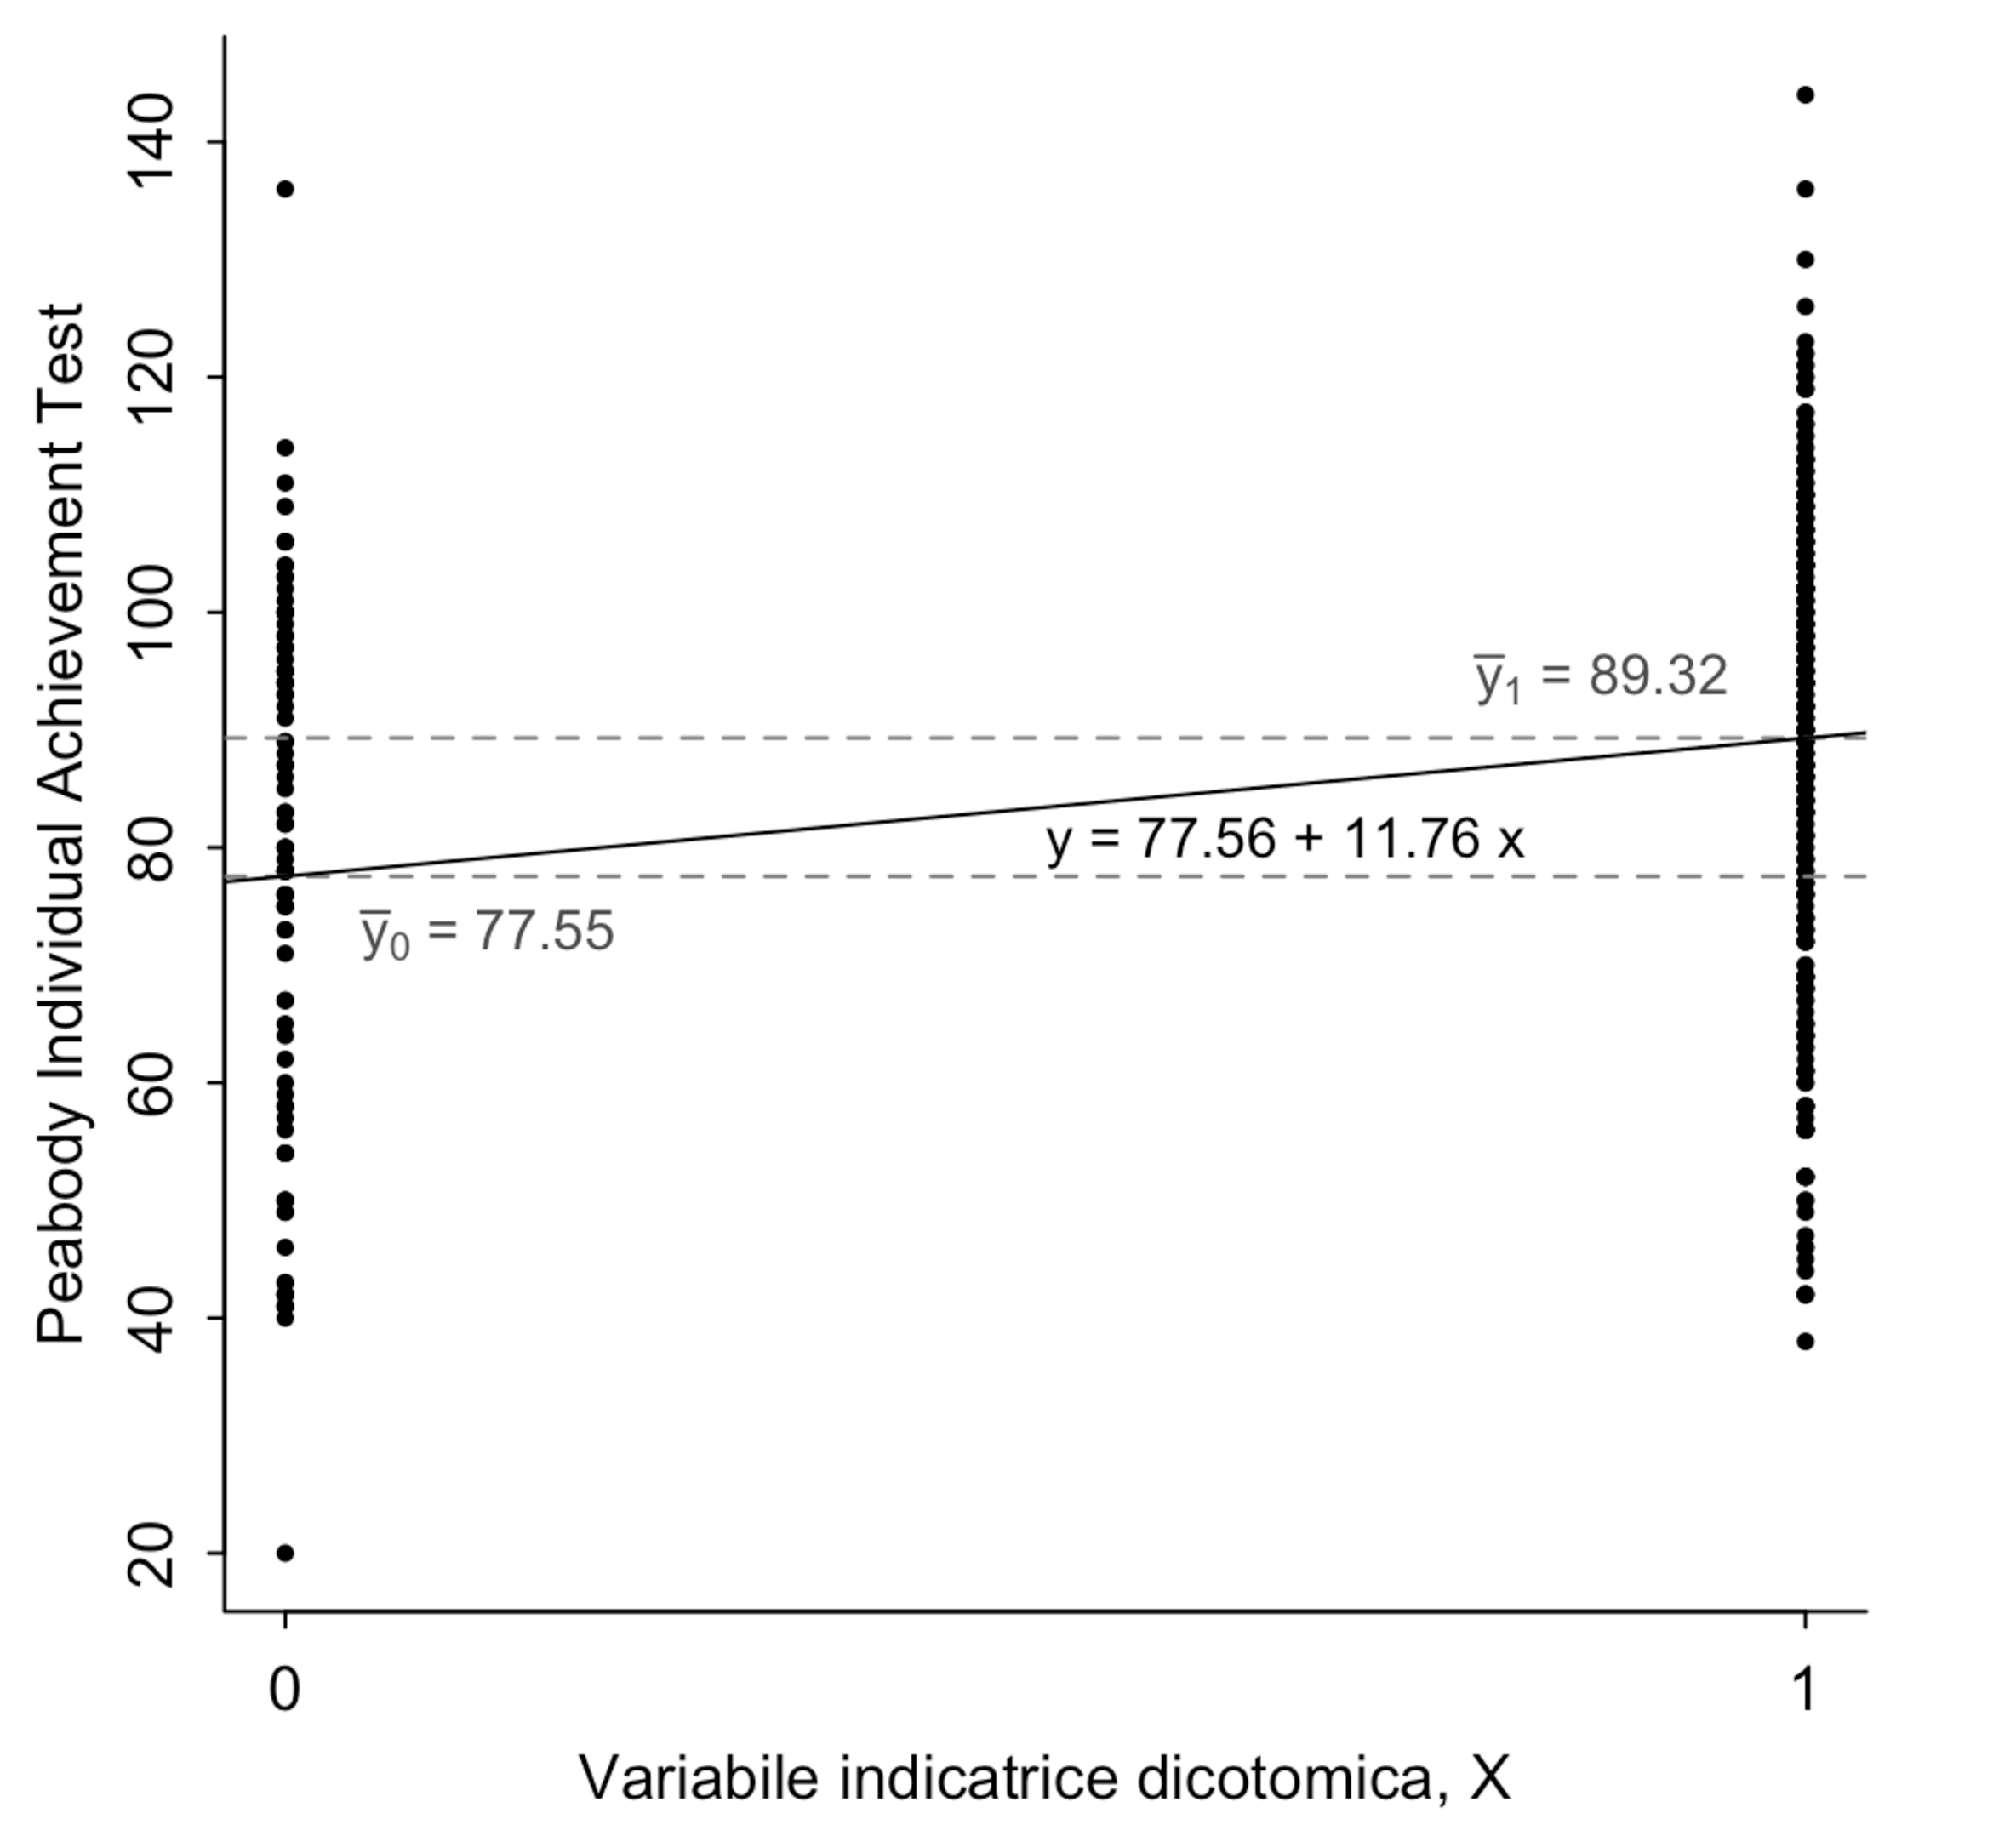
\includegraphics[width=0.7\textwidth]{kid_scores}
 \caption{Distribuzione dei punteggi del \emph{Peabody Individual Achievement Test} in due gruppi di bambini facenti parte del campione discusso da Gelman, Hill, e Vehatari (2020): bambini la cui madre non hanno completato la scuola media superiore ($X$ = 0) e bambini la cui madre ha completato la scuola media superiore ($X$ = 1). 
}
\label{fig:kid_scores}
\end{figure}

Abbiamo visto sopra che il parametro $b$ = 11.77 riflette semplicemente la differenza tra le medie dei due gruppi.
Ma il modello statistico lineare ci dice qualcosa in più: esso quantifica la nostra incertezza relativamente a tale differenza, al di là delle caratteristiche specifiche del particolare campione che abbiamo esaminato. 
È ovvio chiedersi: se esaminassimo un altro campione, quanto sarebbe grande questa differenza?
E in un altro campione ancora?
Il modello statistico lineare ci dice che, indipendentemente da quale campione di dati verrà esaminiamo, ci possiamo aspettare, con un grado di certezza del 95\%, che la differenza tra le medie dei due gruppi sia compresa nell'intervallo tra 7.2 e 16.3 punti PIAT.
Questo è il significato dell'\emph{intervallo di credibilità} al 95\% che è stato calcolato e che ci viene fornito dalla funzione \verb+precis()+.

L'intervallo di credibilità al 95\% rappresenta una stima dell'intervallo di valori che contengono il 95\% dell'area della distribuzione a posteriori del parametro $b$.
Nella figura~\ref{fig:kid_score_mom_hs_post_distr} si vedono le distribuzioni a posteriori dei parametri $a$ e $b$.
Tali distribuzioni sono state generate estraendo un numero molto grande di campioni dalle distribuzioni a posteriori di $a$ e $b$
Solitamente tali stime sono ottenute mediante una variante dell'algoritmo di Metropolis (si veda il capitolo~\ref{chapter:stima_funzione_aposteriori});
% la variante qui utilizzata si chiama campionatore No-U-Turn o Hamilton Monte Carlo.
l'approssimazione quadratica qui usata fornisce un'approssimazione a questo processo.
Dalla figura~\ref{fig:kid_score_mom_hs_post_distr} vediamo che le distribuzioni a posteriori tendono ad essere Normali.
Vediamo inoltre che i valori più plausibili per il parametro $b$ sono compresi tra 7.2 e 16.3, come ci dice l'intervallo di credibilità al 95\%. 
Il problema di come sia possibile specificare un intervallo di credibilità sulla base delle informazioni fornite dalla distribuzione a posteriori è stato discusso nel capitolo~\ref{chapter:riassumere_distr_post}
\footnote{
I metodi di stima MCMC costituiscono la modalità usuale per generare la distribuzione a posteriori nell'analisi Bayesiana.
In queste dispense, però, ci limitiamo ai metodi di stima basati sull'approssimazione quadratica.
Abbiamo deciso di svolgere gli esercizi mediante l'approssimazione quadratica piuttosto che con il metodo MCMC perché l'installazione sul proprio computer del software necessario per le analisi MCMC costituisce un problema di tipo informatico che esula dagli scopi di questo insegnamento.
}.

%\begin{figure}[h!]
% \centering
% \includegraphics[width=\textwidth]{posterior_kid_score_mom_hs}
% \caption{Distribuzione a posteriori dei parametri $a$ (\texttt{b\_Intercept}) e $b$ (\texttt{b\_mom\_hs}) del modello statistico lineare che descrive i punteggi del \emph{Peabody Individual Achievement Test} come funzione del gruppo di appartenenza: i bambini la cui madre non ha completato la scuola media superiore e i bambini la cui madre ha completato la scuola media superiore.
%I dati sono tratti da Gelman, Hill e Vehatari (2020). 
%}
%\label{fig:posterior_kid_score_mom_hs}
%\end{figure}

%Ciò che abbiamo \enquote{guadagnato} eseguendo quest'analisi Bayesiana è l'intervallo di credibilità al 95\% associato al coefficiente $b$.
%In base ad esso possiamo fare l'inferenza che, al di là delle idiosincrasie del particolare campione esaminato, la \enquote{vera} differenza tra le due medie nella popolazione è compresa tra 7.2 e 16.3 punti PIAT.
%Il livello di credibilità al 95\% significa che alla proposizione precedente associamo un livello di certezza del 95\%.

In conclusione, il modello statistico lineare riassume la differenza nei punteggi medi del test PIAT nei due gruppi di bambini: i bambini la cui madre ha completato la scuola media superiore e bambini la cui madre non ha completato la scuola media superiore.
Il modello statistico lineare ci consente inoltre di fare inferenza sulla differenza nei punteggi medi del test PIAT nei due gruppi di bambini.
Viene infatti definito un livello di credibilità che descrive, ad un determinato grado di certezza, quelli che sono i valori plausibili di tale differenza, al di là delle idiosincrasie del particolare campione che abbiamo esaminato, ovvero tenendo in considerazione il fenomeno della variabilità campionaria.
Questo è il processo di inferenza Bayesiana che viene svolta mediante l'uso di un modello statistico lineare.


%--------------------------------------------------------------------
\subsubsection{Quale distribuzione a priori è corretta?}
Un grave problema che è emerso negli anni recenti relativamente all'analisi dei dati psicologici (e non solo) è il cosiddetto \enquote{$p$-hacking}, ovvero la pratica di adattare il modello e i dati allo scopo di ottenere il risultato desiderato. 
Il risultato desiderato è generalmente un valore-$p$ inferiore al 5\%. 
Il problema è che quando il modello statistico viene modificato alla luce dei dati osservati, i valori-$p$ non mantengono più il loro significato originario: in altre parole, il \enquote{$p$-hacking} aumenta la probabilità di ottenere dei risultati falsi. 
L'approccio Bayesiano non prevede i valori-$p$, ma il rischio rimane se scegliamo le distribuzioni a priori in base alle proprietà del campione allo scopo di ottenere il risultato desiderato. 
La procedura che invece deve essere seguita è quella di scegliere le distribuzioni a priori sulla base di considerazioni generali, indipendentemente dalle specifiche caratteristiche del campione.
%, ovvero sulla base di considerazioni generali che possono essere fatte prima di avere eseguito l'esperimento o di avere raccolto i dati. 
% Le distribuzioni a priori devono essere motivate da considerazioni generali, non dal campione. 


%--------------------------------------------------------------------
\section{Una variabile indipendente continua}
\label{sec_var_ind_dico}

Continuiamo ora con l'esempio relativo al \emph{National Longitudinal Survey of Youth} discusso da Gelman et al. (2020). 
Poniamoci il problema di descrivere mediante un modello statistico lineare  l'associazione tra l'intelligenza del bambino, \texttt{kid\_score}, ovvero il punteggio totale del \emph{Peabody Individual Achievement Test} (PIAT), e \texttt{mom\_iq}, ovvero il quoziente di intelligenza della madre (figura~\ref{fig:kid_scores_reg_line}). 

\begin{figure} %[h!]
 \centering
 \includegraphics[width=0.75\textwidth]{kid_scores_reg_line}
 \caption{Punteggio del test PIAT come funzione del QI materno con sovrapposta la linea di regressione. Ogni punto sulla linea di regressione può essere concepito come un punteggio il punteggio predetto per un bambino la cui madri ha il QI corrispondente o come il punteggio PIAT medio per una sottopopolazione di bambini le cui madri hanno tutte quel QI.
I dati sono tratti da Gelman, Hill e Vehatari (2020). 
}
\label{fig:kid_scores_reg_line}
\end{figure}

Il modello statistico lineare diventa:
\begin{align}
Y_i &\sim \mathcal{N}(\mu_i, \sigma) \tag*{[verosimiglianza]}\\
\mu_i &= \alpha + \beta(X_i - \bar{X}) \tag*{[modello lineare]}\\
\alpha &\sim \mathcal{N}(0, \sigma_{\alpha}) \tag*{[distr. a priori per $\alpha$]}\\
\beta &\sim \mathcal{N}(0, \sigma_{\beta}) \tag*{[distr. a priori per $\beta$]}\\
\sigma &\sim \text{Uniforme}(0, 50) \tag*{[distr. a priori per $\sigma$]}
\end{align}
Abbiamo descritto $X$ nei termini degli scostamenti dalla media per fare in modo che il coefficiente $\alpha$ corrisponda al valore atteso della $Y$ in corrispondenza della media di $X$ (quoziente di intelligenza della madre) -- questa è una conseguenza del fatto che la retta di regressione, calcolata in questo modo, passa per il punto $(\bar{X}, \bar{Y})$.
Infatti, avrebbe poco senso chiederci qual è il valore atteso del punteggio PIAT quando il quoziente d'intelligenza della madre è uguale a zero.
%Come in precedenza, la verosimiglianza indica che ciascun valore $Y_i$ (ovvero, \verb+kid_score+) segue una distribuzione Normale.
%Tuttavia, la media della distribuzione di ciascuna osservazione $Y_i$, $\mu_i$, è una funzione lineare della variabile $X$ (ovvero, \verb+mom_iq+):
%\[
%\mu_i = a + b mom_iq.
%\]
%Si assume qui che tutte le distribuzioni Normali di $Y_i$ attorno a $\mu_i$ abbiano la stessa deviazione standard, ovvero $\sigma$.



%In maniera equivalente, possiamo pensare al modello statistico 
%\begin{equation}
%Y_i = \alpha + \beta X_i + \varepsilon_i
%\label{eq:reg_biv}
%\end{equation}
%%il parametro $\alpha$ è l'ordinata all'origine (o intercetta) mentre il parametro $\beta$ è il coefficiente angolare della retta. 
%%Possiamo interpretare l'equazione~\eqref{eq:reg_biv} 
%immaginando che esso descriva la relazione lineare tra le variabili aleatorie $X$ ed $Y$ e che tale relazione lineare sia perturbata da un errore casuale $\varepsilon$, come indicato nella figura~\ref{fig:reg_lin_det_alea}. 
%
%\begin{figure}[h!]
%\centering
%\begin{tikzpicture}[
%  >=stealth,
%  cx/.style={color=black, text width=2cm, font=\footnotesize},
%  pil/.style={->, color=gray, rounded corners},
%  every node/.style={color=black}]
%  \begin{axis}[
%    xticklabels={,,},
%    yticklabels={,,},
%    width=6cm, height=6cm,
%    xlabel=$x$:\, predittore, ylabel=$y$:\, risposta]
%    \addplot[color=gray, thick, mark=none, domain=0:13] {2+3.4*x}
%      node[pos=0.8, sloped, below] {$f(x)=\alpha+\beta x$};
%    \addplot[color=gray, only marks, mark=o]
%      coordinates {
%        (1,8)
%        (2,7)
%        (3,11)
%        (4,20)
%        (5,12)
%        (6,25)
%        (7,24)
%      };
%    \coordinate (pontoreta) at (axis cs: 10, 36);
%    \coordinate (yfit) at (axis cs: 5, 19);
%    \coordinate (yobs) at (axis cs: 5, 12);
%    \node[cx, align=flush right] (compdet)
%      at (axis description cs: 0.35, 0.8)
%      {Componente deterministica ($\hat{y}$)};
%    \draw[pil] (compdet) -| (pontoreta);
%    \draw[pil, <->] (yfit) -- node[cx, right]
%      {Componente aleatoria $(\varepsilon)$} (yobs);
%\end{axis}
%\end{tikzpicture}
%\caption{Relazione statistica lineare tra $X$ e $Y$.}
%\label{fig:reg_lin_det_alea}
%\end{figure}

Specifichiamo dunque il modello statistico lineare con la sintassi richiesta da \verb+rethinking+:




\begin{lstlisting}
flist <- alist(
  kid_score ~ dnorm(mu, sigma),
  mu ~ a + b * (mom_iq - mean(mom_iq)),
  a ~ dnorm(mean(kid_score), 100),
  b ~ dnorm(0, 100),
  sigma ~ dunif(0, 100)
)
\end{lstlisting}
 


Adattiamo il modello lineare ai dati




\begin{lstlisting}
m1 <- quap(
  flist,
  data = df
)
\end{lstlisting}
\noindent
e esaminiamo il risultato ottenuto mediante la funzione \verb+precis()+:
\begin{lstlisting}
precis(m1, prob = 0.95)

#>        mean   sd  2.5% 97.5%
#> a     86.80 0.87 85.08 88.51
#> b      0.61 0.06  0.50  0.72
#> sigma 18.22 0.62 17.01 19.44
\end{lstlisting}
 


Troviamo così che 
\[
\Ev (\text{kid\_score}) = 86 + 0.61 \cdot x,
\]
laddove $x$ è la variabile \verb+kid_score+ espressa come scostamento rispetto al suo valore medio. 
Tale retta di regressione stimata è mostrata assieme ai dati  nella figura~\ref{fig:kid_scores_reg_line}.
Il coefficiente $b$ ci dice che, all'aumentare di un punto del quoziente d'intelligenza della madre, la media dei punteggi PIAT cresce di 0.61 unità.
Il parametro $\sigma$ ci dice che la deviazione standard che quantifica la dispersione dei dati attorno alla retta di regressione è pari a 18.22.

L'intervallo di credibilità di questo coefficiente ci dice che, con un livello di certezza del 95\%, possiamo essere sicuri che, all'aumentare di un punto del quoziente d'intelligenza della madre, la media dei punteggi PIAT crescerà, come minimo, di 0.50 punti e, come massimo, di 0.72 punti.
La differenza 0.72 - 0.50 esprime il nostro grado di incertezza rispetto alla stima del parametro, quando vogliamo che la nostra stima sia \enquote{credibile} al livello di 0.95. 
Ma non c'è niente di \enquote{magico} o necessario relativamente al livello di 0.95.
Infatti, il default della funzione \verb+precis()+ è 0.89.
Ciascuno di questi valori è arbitrario.
Sono possibili tantissime soglie per quantificare la nostra incertezza: alcuni ricercatori usano il livello di 0.5.
Il nostro obiettivo è quello di descrivere il livello della nostra incertezza relativamente alla stima del parametro.
E la nostra incertezza è descritta dall'\emph{intera} distribuzione a posteriori.
Per cui il metodo più semplice, più diretto e più completo per descrivere la nostra incertezza rispetto alla stima dei parametri è quello di riportare graficamente tutta la distribuzione a posteriori, come indicato per esempio nella figura~\ref{fig:posterior_kid_score_mom_iq}.

\begin{figure} %[h!]
 \centering
 \includegraphics[width=\textwidth]{kid_scores_mom_iq}
 \caption{Distribuzione a posteriori dei parametri $a$, $b$ e $\sigma$ del modello statistico lineare che descrive i punteggi del \emph{Peabody Individual Achievement Test} come funzione del quoziente d'intelligenza della madre espresso come scostamento rispetto al suo valore medio.
I dati sono tratti da Gelman, Hill e Vehatari (2020). 
}
\label{fig:posterior_kid_score_mom_iq}
\end{figure}
 

\section{Ipotesi sulla popolazione}

In maniera equivalente, possiamo esprimere il modello statistico lineare descritto sopra elencando le seguenti quattro ipotesi a proposito della struttura della popolazione da cui abbiamo estratto i dati del campione.

\begin{enumerate}
\item La funzione di regressione è lineare (\emph{linearità}):
\begin{equation}
\Ev(y_i \mid x_1, \dots, x_n) = \alpha + \beta x_i, \quad
i=1, \dots, n.
\end{equation}
Le medie delle distribuzioni condizionali $y \mid x_i$ sono linearmente associate alla variabile esplicativa $x$.

\item Le varianze delle distribuzioni condizionali $y \mid x_i$ sono costanti al variare della $x$ (\emph{omoschedasticità}):
\begin{equation}
\var(y_i \mid x_1, \dots,  x_n) = \sigma^2, \quad i=1,
\dots, n. 
\end{equation}

\item Le osservazioni $y_i$ sono tra loro incorrelate subordinatamente alle $x_i$ (\emph{indipendenza}):
\begin{equation}
\cov(y_i, y_j \mid x_1, \dots, x_n) = 0, \quad per \hskip.1 in i \neq j, 
\end{equation}
ovvero, l'osservazione $y_i$ è selezionata dalla distribuzione condizionale $y_i \mid x_i$ tramite un campionamento casuale indipendente.

\item La distribuzione di $y_i$  subordinata a $X=x_i$ segue la distribuzione Normale (\emph{normalità}):
\begin{equation}
(y_i \mid x_i) \sim \mathcal{N}(\alpha+\beta x_i, \sigma^2).
\end{equation}
\end{enumerate}
Il modello statistico lineare può dunque essere rappresentato in forma geometrica come indicato nella figura~\ref{fig:mod_reg_bivariata}.

\begin{figure} % [h!]
\centering

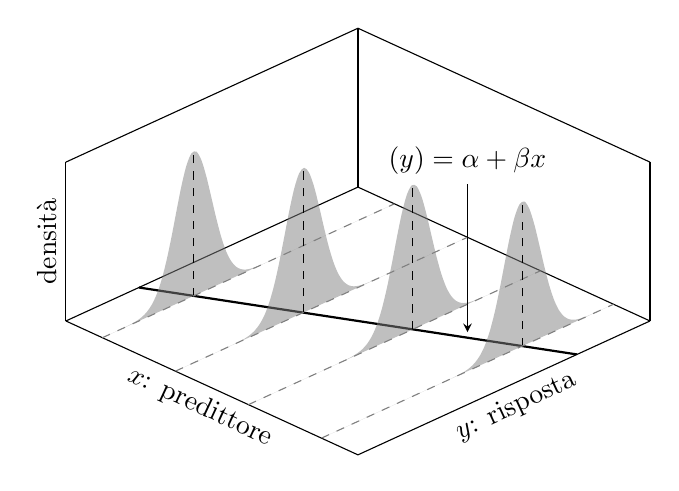
\begin{tikzpicture}[
  >=stealth,
  declare function={
    normal(\m,\s)=1/(2*\s*sqrt(pi))*exp(-(x-\m)^2/(2*\s^2));
  },
  declare function={
    reg(\x,\a,\b)=\a+\b*\x;
  }]

  \begin{axis}[
    width=9cm,
    height=7cm,
    view={45}{50},
    xlabel=$x$: predittore,
    ylabel=$y$: risposta,
    zlabel=densità,
    xlabel style={rotate=-25},
    ylabel style={rotate=25},
    zlabel style={rotate=0},
    samples=60,
    domain=-4:12,
    % title=Regress\~{a}o linear simples,
    % grid=both,
    % minor tick num=2,
    % xtick={1,3,5,7},
    % xticklabel=\empty,
    xtick=\empty,
    ztick=\empty,
    ytick=\empty,
    samples y=0,
    zmin=0,
    area plot/.style={
      fill opacity=0.5,
      draw=none,
      fill=gray,
      mark=none,
      smooth
    }]

    \addplot3[smooth, mark=none, color=black, thick,
      domain=0:8, samples=10] (x,{reg(x,0,1)},0);
    \pgfplotsinvokeforeach{1,3,...,7}{
      \addplot3 [area plot] (#1,x,{normal(#1,1)});
      \draw [dashed] (axis cs:#1,#1,0) -- (axis cs:#1,#1,0.28);
      \draw [gray, dashed] (axis cs:#1,-4,0) -- (axis cs:#1,12,0);
    }
    \draw[<-, shorten <=2pt, shorten >=0pt]
      (axis cs:6,6,0) -- (axis cs:6,6,0.3)
      node[above] {$\Ev(y)=\alpha + \beta x$};
  \end{axis}
\end{tikzpicture}
\caption{Rappresentazione geometrica del modello statistico lineare.}
\label{fig:mod_reg_bivariata}
\end{figure}


\section*{Conclusioni}

Questo capitolo ha introdotto il modello bivariato di regressione lineare, ovvero un metodo che ci consente di stimare l'associazione tra una variabile indipendente e una variabile dipendente. 
La distribuzione Normale può essere usata per specificare la funzione di verosimiglianza in modelli statistici di questo tipo perché può essere concepita come un modo di contare in quanti diversi modi diverse combinazioni di $\mu$ e $\sigma$ possono produrre un'osservazione. 
Per adattare questi modelli ai dati, il presente capitolo ha introdotto un'approssimazione quadratica della distribuzione a posteriori e ha introdotto la funzione \verb+quap()+. 
Sono state inoltre introdotte nuove procedure per visualizzare le distribuzioni a posteriori e per descrivere le stime a posteriori.

Si noti che, per definire la distribuzione a priori del parametro $p$ di una distribuzione di Bernoulli, nella sezione~\ref{sec:idrossi}, abbiamo usato una distribuzione uniforme (a priori non informativa), ovvero Beta(1, 1). 
In tali circostanze, l'intervallo di credibilità è praticamente identico all'intervallo di confidenza di tipo frequentista (si veda il capitolo~\ref{chapter:int_confidence}). 
L'intervallo di credibilità, invece, differisce dall'intervallo di confidenza frequentista quando il modello statistico Bayesiano include una distribuzione a priori informativa o debolmente informativa.
L'analisi dei dati Bayesiana fa quasi sempre uso di distribuzioni a priori debolmente informative, mentre le distribuzioni a priori informative sono più rare.
Le distribuzioni a priori debolmente informative hanno quale scopo la regolarizzazione, cioè, l'obiettivo di mantenere le inferenze in una gamma ragionevole di valori; ciò contribuisce nel contempo a limitare l'influenza eccessiva delle osservazioni estreme (valori anomali).
Alcuni esempi del processo di regolarizzazione sono forniti nella sezione~\ref{sec_mod_lin}. 










